%%%%%%%%%%%%%%%%%%%%%%%%%%%%%%%%%%%%%%%%%%%%%%%%%%%%%%%%%%%%%%%%%%%%%%%%%%%%%%%
%
% Tommy P. Keane
% Master of Science Thesis
% Department of Electrical and Microelectronic Engineering
%
% March 2011
%
%
%
% .tex and .sty modified from:
% http://www.ce.rit.edu/studentresources/gradresource/LaTexThesis.zip
%
%%%%%%%%%%%%%%%%%%%%%%%%%%%%%%%%%%%%%%%%%%%%%%%%%%%%%%%%%%%%%%%%%%%%%%%%%%%%%%%

%%%%%%%%%%%%%%%%%%%%%%%%%%%%%%%%%%%%%%%%%%%%%%%%%%%%%%%%%%%%%%%%%%%%%%%%%%%%%%%
%
% CHAPTER 3
%
% SECTION 1
%
%%%%%%%%%%%%%%%%%%%%%%%%%%%%%%%%%%%%%%%%%%%%%%%%%%%%%%%%%%%%%%%%%%%%%%%%%%%%%%%


%%%%%%%%%%%%%%%%%%%%%%%%%%%%%%%%%%%%%%%%%%%%%%%%%%%%%%%%%%%%%%%%%%%%%%%%%%%%%%%
% BEGIN DOCUMENT

The basic algorithm contains 5 major steps as shown in the flowchart in Figure \ref{algorithmFlowchart} below. This chart shows the processing order of each step, but purposefully has labeled them by their goal and not their specific implementation details. The exact processes of the algorithm will be explained in the following subsections, but, as is the intended purpose of the flowchart, it should be kept in mind that the specific operations were chosen to serve the goals. The overall algorithm itself could be implemented differently as long as the main goals in each step are met. This will be discussed further in Chapter 4.

\begin{figure}
\label{algorithmFlowchart}
\centering
\vskip-.25in
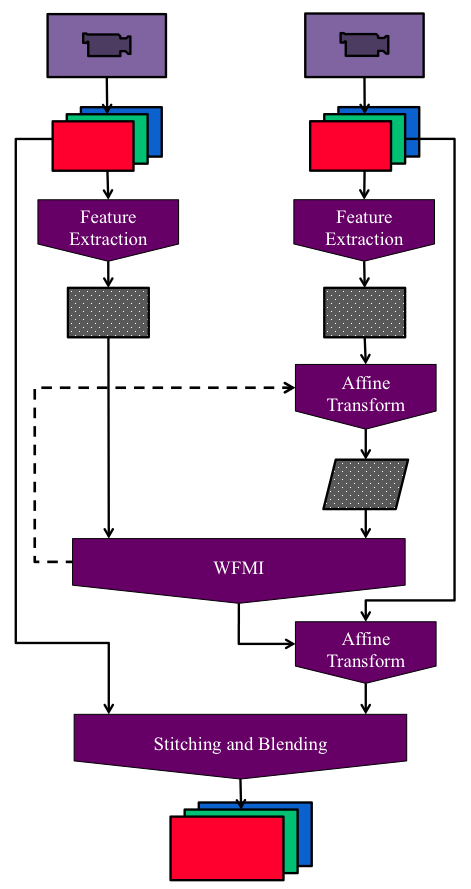
\includegraphics[height=1\textheight]{algorithmFlowchart}
\caption{Flowchart}
\end{figure}


%%%%%%%%%%%%%%%%%%%%%%%%%%%%%%%%%%%%%%%%%%%%%%%%%%%%%%%%%%%%%%%%%%%%%%%%%%%%%%%
% END OF DOCUMENT
